\ifx\wholebook\relax \else

\documentclass[b5paper]{ctexart}
\usepackage[nomarginpar
  %, margin=.5in
]{geometry}

\addtolength{\oddsidemargin}{-0.05in}
\addtolength{\evensidemargin}{-0.05in}
\addtolength{\textwidth}{0.1in}

\usepackage[cn]{../prelude}

\setcounter{page}{1}

\begin{document}

\title{分数}

\author{刘新宇
\thanks{{\bfseries 刘新宇} \newline
  Email: liuxinyu99@hotmail.com \newline}
  }

\maketitle
\fi

\markboth{分数}{数的旅程}

\ifx\wholebook\relax
\chapter{分数}
\fi

\epigraph{此曲只应天上有,人间能得几回闻。}{杜甫《赠花卿》}

2015年9月14日,美国LIGO\footnote{激光干涉引力波}天文台探测到一个神秘信号GW150914。它来自13亿光年之外的一次惊天动地的奇观:一对双黑洞天体彼此靠近、吸引,旋转着合并到一起(如\cref{fig:gravitational-wave})。它们巨大引力激起的“涟漪”穿越13亿年时空\footnote{根据爱因斯坦的广义相对论,引力波以光速传播。}到达了地球。物理学家们花了几个月的事件进行数据分析,排除了可能的干扰因素,最终于2016年2月11日正式宣布:这是人类首次探测到了引力波,证实了爱因斯坦在百年前通过广义相对论做出的预言。LIGO的物理学家们把引力波转换成声音信号,我们得以首次听到来自宇宙深处的“天籁之音”。

\begin{figure}[htbp]
 \centering
 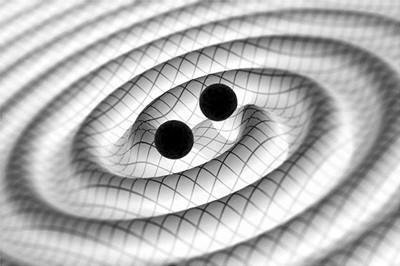
\includegraphics[scale=0.35]{img/gravitational-wave}
 \caption{双黑洞彼此合并过程中产生的引力波示意。}
 \label{fig:gravitational-wave}
\end{figure}

2500年前,正是追寻天籁之音的过程,使得古希腊的先贤毕达哥拉斯发现了音乐背后的数学秘密。相传有一天毕达哥拉斯经过铁匠铺,听到从里面传出了悦耳的声音。这些声音是铁匠用不同重量的铁锤一起敲打铁砧时产生的。毕达哥拉斯注意到有些声音是和谐的,而另一些不和谐。他进一步发现当铁锤的重量比恰好是12、9、8、6时,敲打的声音是和谐的。毕达哥拉斯敏锐地发现了音乐背后的数字规律:

\begin{itemize}
\item 比例$12:6$(即$2:1$)对应纯8度音;
\item 比例$9:6$(即$3:2$)对应纯5度音;
\item 比例$12:9$(即$4:3$)对应纯4度音;
\item 比例$9:8$对应纯2度音。
\end{itemize}

这个故事非常流行。巴洛克时期的音乐家亨德尔有一部作品叫做《快乐的铁匠》(作品编号:HWV430)。但这个故事\underdot{不是真实}的。我们可以通过一个小实验推翻它。用几个同样的杯子盛上不同的水,如

\begin{figure}[htbp]
 \centering
 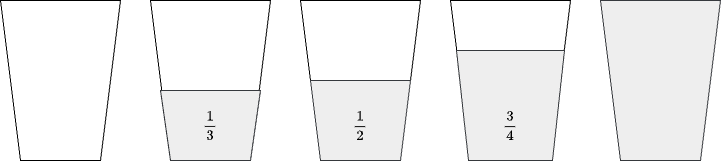
\includegraphics[scale=0.4]{img/cups}
 \caption{盛有不同水的杯子}
 \label{fig:fraction-cups}
\end{figure}

\ifx\wholebook\relax \else
\section{参考答案}
\shipoutAnswer

\begin{thebibliography}{99}
%% \subimport{inc/}{bib-zh-cn}
\end{thebibliography}

\expandafter\enddocument
\fi
